% !TEX program = xelatex
\documentclass{article}
\usepackage[UTF8,fontset=none,scheme=plain]{ctex}
\usepackage[preprint]{icml2026}
\usepackage{fontspec}
\setmainfont{Times New Roman}
\setsansfont{Arial}
\setmonofont{Menlo}[Scale=0.82]
\setCJKmainfont{Songti SC}[BoldFont=Songti SC Bold]
\setCJKsansfont{Heiti SC}
\setCJKmonofont{Heiti SC}
\usepackage{amsmath,amssymb,mathtools,booktabs,array,tabularx,multirow}
\usepackage{graphicx,colortbl,enumitem,microtype,placeins,stfloats,float,balance}
\usepackage[hyperfootnotes=false]{hyperref}
\hypersetup{colorlinks=true,linkcolor=blue!45!black,citecolor=blue!45!black,urlcolor=blue!45!black,pdftitle={数学专用分词器：Benchmark与泛化实验},pdfauthor={肖童仁}}
\setlist[itemize]{leftmargin=1.3em,itemsep=2pt,parsep=0pt,topsep=3pt}
\setlist[enumerate]{leftmargin=1.5em,itemsep=2pt,parsep=0pt,topsep=3pt}
\setlength{\emergencystretch}{1.5em}
\setlength{\tabcolsep}{4pt}
\renewcommand{\arraystretch}{1.12}
\newcolumntype{Y}{>{\raggedright\arraybackslash}X}
\newcommand{\code}[1]{\texttt{\detokenize{#1}}}
\newcommand{\up}{\ensuremath{\uparrow}}
\newcommand{\dn}{\ensuremath{\downarrow}}
\icmltitlerunning{Mathematical Tokenization}
\captionsetup[table]{name=表}
\captionsetup[figure]{name=图}
\captionsetup{labelfont={normalfont,small}}
\makeatletter
\def\fnum@table{表\nobreakspace\thetable}
\def\fnum@figure{图\nobreakspace\thefigure}
\setlength{\@fptop}{0pt}
\setlength{\@fpsep}{10pt}
\setlength{\@fpbot}{0pt plus 1fil}
\setlength{\@dblfptop}{0pt}
\setlength{\@dblfpsep}{10pt}
\setlength{\@dblfpbot}{0pt plus 1fil}
\makeatother
\begin{document}
\raggedbottom
\twocolumn[
\icmltitle{数学专用分词器：Benchmark与泛化实验}
\begin{icmlauthorlist}
\icmlauthor{肖童仁}{author}
\end{icmlauthorlist}
\icmlaffiliation{author}{数学分词器研究项目}
\icmlcorrespondingauthor{肖童仁}{github.com/xtr1976536/math-tokenizer-lab}
\icmlkeywords{Mathematical tokenization, BPE, AST, benchmark, generalization}
\vskip 0.15in
]
\printAffiliationsAndNotice{}
\begin{abstract}
本文构建包含56,000条LaTeX公式的数学分词benchmark，按领域、来源和复杂度分类。我们研究数学原子BPE与软AST-BPE，并与标准AST-BPE及五个基准比较。实验包含领域内、跨领域、极限泛化和简单到复杂四类设置，使用六项指标评价压缩、数学单位完整性、语法跨越、词表使用与编码速度。软AST-BPE在11组划分中均取得最低T/B，领域内相对BPE减少7.45\%的每字节token数，命令完整率为99.73\%。标准AST-BPE的Cross更低，软AST-BPE则获得更好的压缩与编码吞吐。

\end{abstract}
\section{引言}
通用分词器按照文本频率学习子词，数学公式则包含完整控制命令、数字和嵌套参数。本文研究：利用数学词法与语法信号构造专用分词器，能否同时改善公式压缩、数学单位的完整性和编码速度，并迁移到新的数学领域。

我们构建由56,000条LaTeX公式组成的benchmark，比较数学BPE、软AST-BPE、标准AST-BPE与五个基准分词器。实验从领域内、跨领域、极限泛化和简单到复杂四个方面评价分词器，共包含11组划分。本文的主要工作包括：
\begin{itemize}
\item 整理具有来源、领域和复杂度分类的数学公式benchmark，并定义六项评价指标。
\item 设计基于数学原子的BPE和基于软语法约束的AST-BPE，与标准硬约束AST-BPE比较。
\item 在统一语料划分下评价八个分词器，分析压缩、命令完整性、数字完整性、语法跨越和编码速度。
\end{itemize}

\section{相关工作}
\paragraph{词表学习与推理。}
BPE通过高频相邻对合并构建词表\citep{sennrich-etal-2016-neural}。Unigram通过概率估计和剪枝学习子词，并以Viterbi选择分割\citep{kudo-2018-subword,kudo-richardson-2018-sentencepiece}。词表与推理策略可以分别研究：同一词表采用合并顺序或最短路径，会产生不同的分词结果\citep{uzan-etal-2024-greed,schmidt-etal-2024-tokenization}。本文数学BPE和软AST-BPE共享词表，以比较推理阶段的结构引导。

\paragraph{结构引导与分词评价。}
AST-BPE限制合并片段与语法树的层次一致\citep{muller2019ast}；AST-T5利用语法树进行分割和预训练\citep{gong2024ast}。TokEval和跨规模分词研究结合压缩、速度与结构性质评价分词器\citep{meister2026tokeval,lotz-etal-2025-beyond}。数字分组也会影响算术计算\citep{singh2024counts}。本文集中评价数学公式的六项内在指标，并比较数学原子、硬语法约束和软语法约束。

\section{Benchmark}
\subsection{数据来源与分类}
benchmark包含56,000条LaTeX公式，覆盖13个公式领域。来源包括283篇2020年前arXiv论文、11篇公开仓库论文和72个公式资源模块。
\begin{table}[H]\centering\small
\caption{Benchmark的公式来源与数量。}\label{tab:sources}
\begin{tabularx}{\columnwidth}{Yr}\toprule 来源&公式数\\\midrule
\href{https://arxiv.org/}{2020年前arXiv论文}&51,229\\
\href{https://github.com/openai/math}{OpenAI数学仓库}&2,810\\
\href{https://github.com/fredrik-johansson/fungrim}{FunGrim}&1,889\\
\href{https://github.com/sympy/sympy}{SymPy}&72\\\midrule
合计&56,000\\\bottomrule\end{tabularx}\end{table}


语料构建分为四步：
\begin{enumerate}
\item 获取固定版本的论文源文件或公式资源，提取数学环境。
\item 展开局部宏，检查公式语法与宏展开后的渲染一致性。
\item 去重并保存来源链接、版本、许可和原始位置。
\item 按数学领域、公式类型、来源标签和复杂度分类。
\end{enumerate}

\begin{table}[H]\centering\small\caption{按公式内容划分的领域分布。}\label{tab:domains}\begin{tabular}{lr@{\quad}lr}\toprule 领域&数量&领域&数量\\\midrule
分析 & 20,233 & 概率 & 3,171\\
几何拓扑 & 9,135 & 统计 & 1,056\\
组合 & 5,563 & 逻辑 & 662\\
代数 & 4,431 & PDE & 356\\
数论 & 4,273 & ODE & 46\\
数学物理 & 3,850 & 线性代数 & 13\\
优化 & 3,211 &  & \\
\bottomrule\end{tabular}\end{table}

来源标签为历史人工、可能混合和未知，分别对应51,229、2,810和1,961条公式。公式类型包括恒等式与界、求和／乘积、积分、多行公式、矩阵和微分关系。论文领域另行记录，用于跨领域划分。

\subsection{公式复杂度}
复杂度使用五个量：词素数$L$、命令种类$C$、括号嵌套深度$D$、符号种类$S$和运算符数$O$。令$r(t)=\min(t,2)$，定义
\begin{equation}\label{eq:complexity}
\begin{aligned}
K(x)={}&0.40r(L/60)+0.20r(C/6)\\
       &+0.15r(D/3)+0.15r(S/18)\\
       &+0.10r(O/12).
\end{aligned}
\end{equation}
$K(x)<0.65$为简单公式，否则为复杂公式；两类分别有37,400和18,600条。
例如，语料中的公式$s^{\frac{1}{3}}$：
\begin{itemize}
\item 源码为\texttt{s\textasciicircum{}\{\textbackslash{}frac\{1\}\{3\}\}}，词素数$L=11$。
\item 只有\code{\frac}一种命令，$C=1$；括号嵌套深度$D=2$。
\item 非括号符号为$s$、\code{^}、\code{\frac}、1、3，故$S=5$；运算符为\code{^}和\code{\frac}，$O=2$。
\end{itemize}
代入式\eqref{eq:complexity}：
\[
\begin{aligned}
K={}&0.40\frac{11}{60}+0.20\frac{1}{6}+0.15\frac{2}{3}\\
&+0.15\frac{5}{18}+0.10\frac{2}{12}\\
={}&0.265<0.65,
\end{aligned}
\]
因此该公式属于简单类。


\subsection{评价指标}
\begin{table}[H]\centering\footnotesize
\caption{测试公式的实际分词。竖线表示token边界。}\label{tab:example}
\begin{tabularx}{\columnwidth}{lY}\toprule 模型&token序列\\\midrule
\multicolumn{2}{l}{A：$x>\frac{2}n$}\\[2pt]
AST-BPE & \texttt{x} $|$\allowbreak \texttt{>} $|$\allowbreak \texttt{\textbackslash{}frac} $|$\allowbreak \texttt{\{2\}} $|$\allowbreak \texttt{n}\\
软AST-BPE & \texttt{x} $|$\allowbreak \texttt{>} $|$\allowbreak \texttt{\textbackslash{}frac\{} $|$\allowbreak \texttt{2\}} $|$\allowbreak \texttt{n}\\
Qwen2.5 & \texttt{x} $|$\allowbreak \texttt{>\textbackslash{}} $|$\allowbreak \texttt{frac} $|$\allowbreak \texttt{\{} $|$\allowbreak \texttt{2} $|$\allowbreak \texttt{\}} $|$\allowbreak \texttt{n}\\
\midrule
\multicolumn{2}{l}{B：$y_{m,n}(1)\geq C_{12}$}\\[2pt]
AST-BPE & \texttt{y\_} $|$\allowbreak \texttt{\{m} $|$\allowbreak \texttt{,} $|$\allowbreak \texttt{n\}} $|$\allowbreak \texttt{(1} $|$\allowbreak \texttt{)} $|$\allowbreak \texttt{\textbackslash{}geq } $|$\allowbreak \texttt{C\_} $|$\allowbreak \texttt{\{} $|$\allowbreak \texttt{12} $|$\allowbreak \texttt{\}}\\
软AST-BPE & \texttt{y} $|$\allowbreak \texttt{\_\{m} $|$\allowbreak \texttt{,} $|$\allowbreak \texttt{n\}} $|$\allowbreak \texttt{(1} $|$\allowbreak \texttt{)} $|$\allowbreak \texttt{\textbackslash{}geq } $|$\allowbreak \texttt{C} $|$\allowbreak \texttt{\_\{1} $|$\allowbreak \texttt{2\}}\\
Qwen2.5 & \texttt{y} $|$\allowbreak \texttt{\_\{} $|$\allowbreak \texttt{m} $|$\allowbreak \texttt{,n} $|$\allowbreak \texttt{\}(} $|$\allowbreak \texttt{1} $|$\allowbreak \texttt{)\textbackslash{}} $|$\allowbreak \texttt{ge} $|$\allowbreak \texttt{q} $|$\allowbreak \texttt{ C} $|$\allowbreak \texttt{\_\{} $|$\allowbreak \texttt{1} $|$\allowbreak \texttt{2} $|$\allowbreak \texttt{\}}\\
\bottomrule\end{tabularx}
\end{table}

我们采用T/B、Cmd、Num、Cross、Used和编码速度六项指标，以下按表\ref{tab:example}的实际分词计算。
\paragraph{T/B $\dn$：压缩。}
单式T/B等于token数除以原串字节数。表\ref{tab:example}的公式A有11字节，软AST-BPE与AST-BPE均分成5个token：
\[\mathrm{T/B}_A=5/11\approx0.4545.\]
Qwen2.5使用7个token，对应$7/11\approx0.6364$。实验表先计算每个来源组的总token数／总字节数，再对来源组取平均：
\[\mathrm{T/B}=\frac{1}{G}\sum_{g=1}^G\frac{T_g}{B_g}.\]

\paragraph{Cmd $\up$：命令完整率。}
公式A只有一个命令\code{\frac}。AST-BPE和软AST-BPE均未在命令内部切开，Cmd为$1/1=100\%$；Qwen2.5将反斜杠与\code{frac}分开，Cmd为$0/1=0\%$。汇总时用完整命令数除以命令总数。

\paragraph{Num $\up$：数字完整率。}
公式B含数字1和12。AST-BPE保留两个数字，Num为$2/2=100\%$；软AST-BPE在12内部切开，Num为$1/2=50\%$。汇总时用内部未切开的数字词素数除以数字词素总数。

\paragraph{Cross $\dn$：语法部分跨越率。}
按KaTeX语法跨度判断token是否部分越过节点。公式A的软AST-BPE将\code{\frac}与左花括号合并，5个token中有1个跨越分子组起点：
\[\mathrm{Cross}_A=1/5\times100\%=20\%.\]
AST-BPE保留分子组，Cross为$0/5=0\%$。实验表用跨越token数除以全部token数，每个token最多计一次。

\paragraph{Used：词表使用率。}
统计输入中出现过的不同ID，除以词表大小：
\[\mathrm{Used}=\frac{\text{已使用的不同ID数}}{\text{词表ID总数}}\times100\%.\]
公式B在软AST-BPE下使用10个不同ID，因此单式Used为$10/1024\times100\%=0.9766\%$。该组完整测试集使用696个ID，Used为$696/1024\times100\%=67.97\%$。
\paragraph{速度 $\up$：完整编码吞吐。}
用原始输入MiB除以完整编码时间：
\[\mathrm{Speed}=\frac{\text{输入字节数}/2^{20}}{\text{编码秒数}}.\]
同组公式A、B所在的完整测试集有659,113字节；软AST-BPE七轮编码的中位耗时为0.02121125秒：
\[\mathrm{Speed}=\frac{659113/2^{20}}{0.02121125}\approx29.63\ \mathrm{MiB/s}.\]
计时包含原子映射、解析和分割，模型加载与指标计算在计时之外。


\section{分词器}
比较模型包括三个数学分词器和五个基准。五个在本语料上训练的模型均使用1,024个ID；Qwen2.5、Llama 3和o200k采用官方完整词表。

\subsection{AST-BPE}
AST-BPE采用\citet{muller2019ast}的硬约束合并原则。数学前端提取算术、分式、根式、括号和上下标的结构跨度，其他命令采用参数绑定结构。
\begin{enumerate}
\item 从字节序列出发，统计与语法层次兼容的相邻token对。
\item 选择频率最高的合法对合并，更新计数，直至词表达到1,024。
\item 推理时按学习到的规则顺序合并，并对每次合并施加同样的硬约束。
\end{enumerate}
若token区间$[a,b)$与节点$[u,v)$满足$a<u<b<v$或$u<a<v<b$，该合并被禁止。例如表\ref{tab:example}中的\code{\frac}和分子组分别保留，避免把命令末尾与分子组开头合在一起。

\subsection{数学BPE}
数学BPE在基础字母表中保护完整数学命令，再使用官方BPE学习词表和执行分词。
\begin{enumerate}
\item 从训练集选取至多384个高频控制命令和非ASCII字符，加上256个基础字节。
\item 将已选完整命令映射为单个基础符号，使用Hugging Face BPE训练到1,024个ID。
\item 推理先执行相同原子映射，再调用官方BPE。原子内部保持完整，原子之间可以合并。
\end{enumerate}

\subsection{软AST-BPE}
软AST-BPE与数学BPE共享词表，在候选分割上加入语法代价。设$T(z)$为token数，$C(z)$为跨越前端语法跨度的token数，$H(z)$为被token覆盖的花括号组内容端点数，目标为
\begin{equation}\label{eq:soft}
z^*=\arg\min_z\bigl[T(z)+0.25C(z)+0.30H(z)\bigr].
\end{equation}
\begin{enumerate}
\item 用trie查找当前位置可用的词表片段。
\item 为每个候选片段计算token代价和结构代价。
\item 用动态规划求总代价最小的分割。解析、匹配和路径搜索由原生C实现完成。
\end{enumerate}
表\ref{tab:example}中，软约束允许命令与左花括号合并；数学命令内部仍由原子约束保护。

\subsection{基准分词器}
\begin{itemize}
\item \textbf{BPE：}Hugging Face字节BPE；256个基础字节计入1,024个ID。
\item \textbf{Unigram：}SentencePiece通过EM与候选剪枝学习词表，推理采用Viterbi。使用identity归一化、byte fallback和原始空白。
\item \textbf{Qwen2.5：}千问2.5系列官方分词器，151,665个ID。
\item \textbf{Llama 3：}Meta Llama 3官方分词器，128,256个ID。
\item \textbf{o200k：}官方tiktoken编码，200,019个ID。
\end{itemize}
\begin{table}[t]\centering\small\caption{模型容量与代码来源。AST-BPE采用公开算法的数学迁移实现。}\label{tab:models}\begin{tabular}{lrr}\toprule 模型&ID空间&来源\\\midrule
AST-BPE & 1,024 & \href{https://github.com/SamuelGabriel/sqlbpe}{代码}\\
软AST-BPE & 1,024 & \href{https://github.com/xtr1976536/math-tokenizer-lab}{代码}\\
数学BPE & 1,024 & \href{https://github.com/huggingface/tokenizers}{代码}\\
BPE & 1,024 & \href{https://github.com/huggingface/tokenizers}{代码}\\
Unigram & 1,024 & \href{https://github.com/google/sentencepiece}{代码}\\
Qwen2.5 & 151,665 & \href{https://huggingface.co/Qwen/Qwen2.5-0.5B/blob/main/tokenizer.json}{代码}\\
Llama 3 & 128,256 & \href{https://github.com/meta-llama/llama3/blob/main/llama/tokenizer.py}{代码}\\
o200k & 200,019 & \href{https://github.com/openai/tiktoken}{代码}\\
\bottomrule\end{tabular}\end{table}


\section{实验}
\subsection{实验设置}
每次划分以整篇论文或资源模块为来源组，清除训练、验证和测试之间的模板及渲染重复。训练集用于学习词表；验证公式不进入词表。词表大小、原子预算和式\eqref{eq:soft}的权重在所有实验中保持一致。
\begin{itemize}
\item \textbf{领域内：}各领域均参与训练和测试，按来源组约80\%／10\%／10\%划分，重复三次。
\item \textbf{跨领域：}每次完整留出三个学科，用其他学科训练，共三个留出组合。
\item \textbf{极限泛化：}分析／PDE／ODE与代数／数论／线性代数两个学科族双向迁移。
\item \textbf{简单到复杂：}只用简单公式训练，在独立来源的复杂公式上测试，重复三次。
\end{itemize}
\begin{table*}[t]\centering\small\caption{四类实验的实际公式数量。跨领域行名表示测试领域；极限泛化行名表示迁移方向。}\label{tab:splits}\begin{tabular}{llrrr}\toprule 实验&划分／测试领域&训练&验证&测试\\\midrule
领域内 & 划分1 & 44,070 & 4,656 & 7,022\\
领域内 & 划分2 & 43,262 & 8,317 & 4,184\\
领域内 & 划分3 & 44,515 & 5,516 & 5,725\\
\addlinespace
跨领域 & 几何／组合／数论 & 31,684 & 5,214 & 18,622\\
跨领域 & 概率／统计／优化 & 42,081 & 6,357 & 7,334\\
跨领域 & 分析／PDE／ODE & 31,313 & 4,022 & 20,259\\
\addlinespace
极限泛化 & 分析方程→代数 & 16,893 & 3,298 & 8,576\\
极限泛化 & 代数→分析方程 & 7,707 & 1,002 & 20,420\\
\addlinespace
简单到复杂 & 划分1 & 29,863 & 3,032 & 2,769\\
简单到复杂 & 划分2 & 29,119 & 5,347 & 1,487\\
简单到复杂 & 划分3 & 29,347 & 3,768 & 1,684\\
\bottomrule\end{tabular}\end{table*}


\subsection{实验结果}
表\ref{tab:id}至表\ref{tab:complexity}依次给出四个实验的完整结果。领域内、跨领域和简单到复杂分别对三个设置取平均，极限泛化对两个方向取平均；每次划分的结果见附录。Cmd、Num、Cross和Used以百分数表示，速度单位为MiB/s。
\begin{table}[H]
\centering\fontsize{8}{9.4}\selectfont\setlength{\tabcolsep}{2.0pt}\renewcommand{\arraystretch}{1.06}
\caption{领域内实验：三个来源划分的均值。}\label{tab:id}
\begin{tabular}{lrrrrrr}\toprule
模型&T/B $\dn$&Cmd $\up$&Num $\up$&Cross $\dn$&Used&速度 $\up$\\\midrule
AST-BPE & 0.4181 & 92.28 & 96.87 & \textbf{7.71} & 74.74 & 14.81 \\
软AST-BPE & \textbf{0.3799} & \textbf{99.73} & 96.37 & 17.50 & 67.97 & \textbf{29.36} \\
数学BPE & 0.3830 & \textbf{99.73} & 96.37 & 18.18 & 68.03 & 10.00 \\
BPE & 0.4105 & 36.27 & 96.37 & 25.17 & 78.26 & 8.49 \\
Unigram & 0.4783 & 4.18 & 97.42 & 19.80 & 71.65 & 23.76 \\
\midrule
Qwen2.5 & 0.5261 & 2.02 & 96.37 & 19.98 & 1.02 & 3.15 \\
Llama 3 & 0.5228 & 2.02 & \textbf{99.23} & 20.14 & 1.30 & 9.00 \\
o200k & 0.5174 & 2.62 & \textbf{99.23} & 20.58 & 0.81 & 14.28 \\
\bottomrule\end{tabular}
\end{table}

\begin{table}[H]
\centering\fontsize{8}{9.4}\selectfont\setlength{\tabcolsep}{2.0pt}\renewcommand{\arraystretch}{1.06}
\caption{跨领域实验：三个留出组合的均值。}\label{tab:ood}
\begin{tabular}{lrrrrrr}\toprule
模型&T/B $\dn$&Cmd $\up$&Num $\up$&Cross $\dn$&Used&速度 $\up$\\\midrule
AST-BPE & 0.4287 & 91.60 & 97.54 & \textbf{7.32} & 75.88 & 14.67 \\
软AST-BPE & \textbf{0.3869} & \textbf{99.70} & 97.08 & 17.26 & 71.39 & \textbf{27.80} \\
数学BPE & 0.3908 & \textbf{99.70} & 97.08 & 17.79 & 71.48 & 9.39 \\
BPE & 0.4161 & 46.20 & 97.08 & 23.47 & 79.49 & 7.73 \\
Unigram & 0.4890 & 3.09 & 97.92 & 19.49 & 72.56 & 22.57 \\
\midrule
Qwen2.5 & 0.5238 & 2.10 & 97.08 & 19.54 & 1.38 & 3.17 \\
Llama 3 & 0.5211 & 2.10 & \textbf{99.36} & 19.66 & 1.90 & 8.80 \\
o200k & 0.5169 & 2.52 & \textbf{99.36} & 20.04 & 1.19 & 14.01 \\
\bottomrule\end{tabular}
\end{table}

\begin{table}[H]
\centering\fontsize{8}{9.4}\selectfont\setlength{\tabcolsep}{2.0pt}\renewcommand{\arraystretch}{1.06}
\caption{极限泛化实验：两个迁移方向的均值。}\label{tab:extreme}
\begin{tabular}{lrrrrrr}\toprule
模型&T/B $\dn$&Cmd $\up$&Num $\up$&Cross $\dn$&Used&速度 $\up$\\\midrule
AST-BPE & 0.4374 & 87.14 & 96.10 & \textbf{7.30} & 75.44 & 15.10 \\
软AST-BPE & \textbf{0.3919} & \textbf{98.58} & 95.29 & 16.59 & 74.61 & \textbf{27.98} \\
数学BPE & 0.3967 & \textbf{98.58} & 95.29 & 16.94 & 74.46 & 9.56 \\
BPE & 0.4286 & 45.84 & 95.34 & 21.52 & 77.05 & 7.71 \\
Unigram & 0.5019 & 3.38 & 96.39 & 18.80 & 71.34 & 22.21 \\
\midrule
Qwen2.5 & 0.5265 & 1.95 & 95.28 & 19.22 & 1.40 & 3.13 \\
Llama 3 & 0.5219 & 1.95 & \textbf{99.01} & 19.40 & 1.98 & 8.76 \\
o200k & 0.5183 & 2.54 & \textbf{99.01} & 19.71 & 1.25 & 14.30 \\
\bottomrule\end{tabular}
\end{table}

\begin{table}[H]
\centering\fontsize{8}{9.4}\selectfont\setlength{\tabcolsep}{2.0pt}\renewcommand{\arraystretch}{1.06}
\caption{简单到复杂实验：三个来源划分的均值。}\label{tab:complexity}
\begin{tabular}{lrrrrrr}\toprule
模型&T/B $\dn$&Cmd $\up$&Num $\up$&Cross $\dn$&Used&速度 $\up$\\\midrule
AST-BPE & 0.4226 & 86.17 & 96.91 & \textbf{7.63} & 73.11 & 16.38 \\
软AST-BPE & \textbf{0.3802} & \textbf{99.62} & 96.13 & 17.96 & 67.25 & \textbf{36.33} \\
数学BPE & 0.3852 & \textbf{99.62} & 96.13 & 19.16 & 67.06 & 11.88 \\
BPE & 0.4084 & 64.80 & 96.13 & 21.50 & 76.89 & 9.56 \\
Unigram & 0.5020 & 2.72 & 97.42 & 16.00 & 67.84 & 29.80 \\
\midrule
Qwen2.5 & 0.5142 & 2.73 & 96.13 & 20.40 & 0.87 & 3.47 \\
Llama 3 & 0.5110 & 2.73 & \textbf{99.14} & 20.58 & 1.09 & 10.12 \\
o200k & 0.5058 & 3.29 & \textbf{99.14} & 21.09 & 0.68 & 16.31 \\
\bottomrule\end{tabular}
\end{table}

\FloatBarrier
\subsection{结果分析}
\begin{itemize}
\item \textbf{压缩：}软AST-BPE在11组划分中均取得最低T/B；四类实验相对BPE分别减少7.45\%、7.02\%、8.54\%和6.91\%。
\item \textbf{命令与数字：}领域内实验中，软AST-BPE和数学BPE的Cmd均为99.73\%，BPE为36.27\%；Llama 3和o200k的Num均为99.23\%，高于数学专用模型。
\item \textbf{结构与速度：}AST-BPE的Cross为7.71\%，软AST-BPE为17.50\%；硬约束产生更少部分跨越。软AST-BPE速度为29.36 MiB/s，数学BPE为10.00 MiB/s。
\end{itemize}

\begin{figure*}[t]\centering
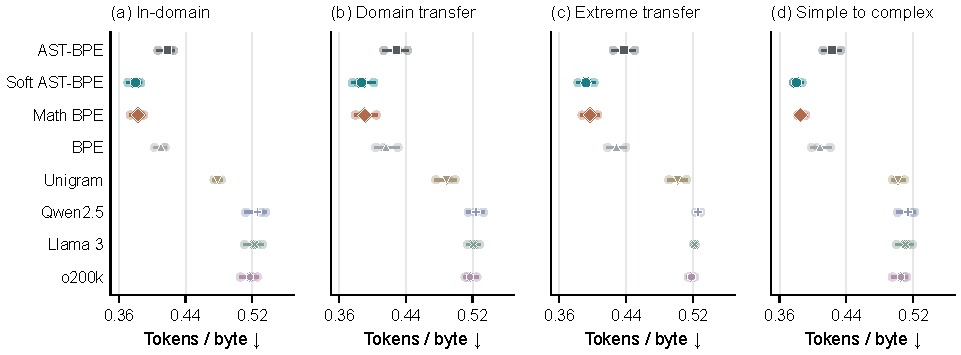
\includegraphics[width=\textwidth]{figures/compression.pdf}
\caption{四类实验的T/B。小点为各次来源划分或迁移设置，线段为范围，大标记为等权均值；每列分别包含3、3、2、3组设置。}\label{fig:compression}
\end{figure*}
\begin{figure*}[t]\centering
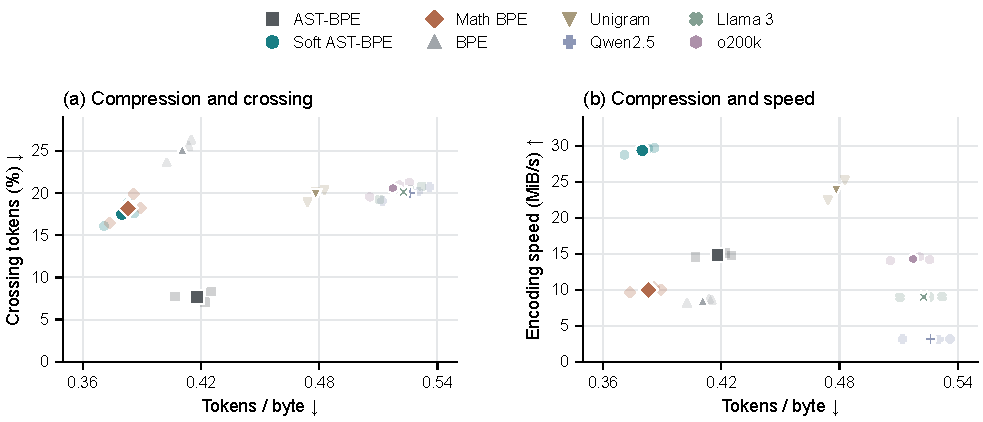
\includegraphics[width=\textwidth]{figures/tradeoffs.pdf}
\caption{领域内三个来源划分的压缩、Cross与编码速度。小点为单次划分，大标记为均值。左图比较压缩与语法跨越，右图比较完整编码接口吞吐。}\label{fig:tradeoffs}
\end{figure*}

\section{结论}
本文构建了具有领域、来源和复杂度分类的数学公式benchmark，并用四类泛化实验比较八个分词器。数学BPE通过完整命令原子改善数学单位表示；软AST-BPE在共享词表上加入结构代价，在11组划分中均获得最低T/B，领域内命令完整率为99.73\%，编码速度为29.36 MiB/s。标准AST-BPE取得更低Cross，显示硬约束与软约束各自的结构与压缩优势。


\clearpage
\balance
\bibliographystyle{icml2026}
\bibliography{references}
\clearpage\appendix\onecolumn
\section{各次划分的结果}
各表沿用正文的六项指标。领域内和简单到复杂实验使用三个来源划分；跨领域实验采用三个留出组合；极限泛化分别报告两个迁移方向。
\begin{table}[H]
\centering\small\renewcommand{\arraystretch}{1.05}
\caption{领域内：划分1。}\label{tab:detail1}
\begin{tabular}{lrrrrrr}\toprule
模型&T/B $\dn$&Cmd $\up$&Num $\up$&Cross $\dn$&Used&速度 $\up$\\\midrule
AST-BPE & 0.4253 & 92.92 & 98.14 & \textbf{8.32} & 75.00 & 14.77 \\
软AST-BPE & \textbf{0.3829} & \textbf{99.92} & 97.63 & 18.85 & 67.97 & \textbf{29.63} \\
数学BPE & 0.3860 & \textbf{99.92} & 97.63 & 19.87 & 68.16 & 10.34 \\
BPE & 0.4152 & 38.04 & 97.63 & 26.31 & 78.71 & 8.59 \\
Unigram & 0.4827 & 4.16 & 98.38 & 20.32 & 71.00 & 25.26 \\
\midrule
Qwen2.5 & 0.5360 & 2.54 & 97.63 & 20.70 & 1.04 & 3.17 \\
Llama 3 & 0.5320 & 2.54 & \textbf{98.67} & 20.81 & 1.31 & 9.05 \\
o200k & 0.5257 & 2.92 & \textbf{98.67} & 21.24 & 0.81 & 14.19 \\
\bottomrule\end{tabular}
\end{table}

\begin{table}[H]
\centering\small\renewcommand{\arraystretch}{1.05}
\caption{领域内：划分2。}\label{tab:detail2}
\begin{tabular}{lrrrrrr}\toprule
模型&T/B $\dn$&Cmd $\up$&Num $\up$&Cross $\dn$&Used&速度 $\up$\\\midrule
AST-BPE & 0.4220 & 91.85 & 95.77 & \textbf{7.05} & 74.22 & 15.11 \\
软AST-BPE & \textbf{0.3861} & \textbf{99.37} & 95.43 & 17.57 & 66.80 & \textbf{29.70} \\
数学BPE & 0.3894 & \textbf{99.37} & 95.43 & 18.23 & 66.99 & 10.02 \\
BPE & 0.4138 & 38.62 & 95.43 & 25.58 & 76.95 & 8.75 \\
Unigram & 0.4782 & 3.87 & 96.53 & 20.15 & 71.29 & 23.56 \\
\midrule
Qwen2.5 & 0.5304 & 2.02 & 95.43 & 20.19 & 0.89 & 3.12 \\
Llama 3 & 0.5257 & 2.02 & \textbf{99.33} & 20.43 & 1.17 & 9.00 \\
o200k & 0.5206 & 2.36 & \textbf{99.33} & 20.96 & 0.74 & 14.59 \\
\bottomrule\end{tabular}
\end{table}

\begin{table}[H]
\centering\small\renewcommand{\arraystretch}{1.05}
\caption{领域内：划分3。}\label{tab:detail3}
\begin{tabular}{lrrrrrr}\toprule
模型&T/B $\dn$&Cmd $\up$&Num $\up$&Cross $\dn$&Used&速度 $\up$\\\midrule
AST-BPE & 0.4069 & 92.07 & 96.71 & \textbf{7.75} & 75.00 & 14.54 \\
软AST-BPE & \textbf{0.3709} & \textbf{99.92} & 96.06 & 16.07 & 69.14 & \textbf{28.74} \\
数学BPE & 0.3737 & \textbf{99.92} & 96.06 & 16.44 & 68.95 & 9.65 \\
BPE & 0.4027 & 32.14 & 96.06 & 23.62 & 79.10 & 8.15 \\
Unigram & 0.4741 & 4.52 & 97.34 & 18.93 & 72.66 & 22.47 \\
\midrule
Qwen2.5 & 0.5120 & 1.51 & 96.06 & 19.05 & 1.13 & 3.15 \\
Llama 3 & 0.5106 & 1.51 & \textbf{99.70} & 19.19 & 1.41 & 8.94 \\
o200k & 0.5057 & 2.56 & \textbf{99.70} & 19.53 & 0.87 & 14.05 \\
\bottomrule\end{tabular}
\end{table}

\begin{table}[H]
\centering\small\renewcommand{\arraystretch}{1.05}
\caption{跨领域：几何／组合／数论。}\label{tab:detail4}
\begin{tabular}{lrrrrrr}\toprule
模型&T/B $\dn$&Cmd $\up$&Num $\up$&Cross $\dn$&Used&速度 $\up$\\\midrule
AST-BPE & 0.4420 & 90.15 & 95.91 & \textbf{6.29} & 77.25 & 14.61 \\
软AST-BPE & \textbf{0.4016} & \textbf{99.50} & 95.60 & 17.66 & 74.51 & \textbf{25.80} \\
数学BPE & 0.4047 & \textbf{99.50} & 95.60 & 18.36 & 74.51 & 8.54 \\
BPE & 0.4305 & 26.77 & 95.60 & 23.81 & 79.98 & 7.09 \\
Unigram & 0.4919 & 3.40 & 96.37 & 20.11 & 73.93 & 20.52 \\
\midrule
Qwen2.5 & 0.5330 & 2.18 & 95.60 & 19.92 & 1.52 & 3.03 \\
Llama 3 & 0.5281 & 2.18 & \textbf{99.31} & 20.11 & 2.27 & 8.41 \\
o200k & 0.5251 & 2.79 & \textbf{99.31} & 20.37 & 1.43 & 13.44 \\
\bottomrule\end{tabular}
\end{table}

\begin{table}[H]
\centering\small\renewcommand{\arraystretch}{1.05}
\caption{跨领域：概率／统计／优化。}\label{tab:detail5}
\begin{tabular}{lrrrrrr}\toprule
模型&T/B $\dn$&Cmd $\up$&Num $\up$&Cross $\dn$&Used&速度 $\up$\\\midrule
AST-BPE & 0.4305 & 91.04 & 98.80 & \textbf{7.85} & 74.32 & 14.87 \\
软AST-BPE & \textbf{0.3831} & \textbf{99.81} & 98.26 & 16.90 & 69.24 & \textbf{29.41} \\
数学BPE & 0.3881 & \textbf{99.81} & 98.26 & 17.30 & 69.34 & 10.46 \\
BPE & 0.4138 & 53.05 & 98.26 & 23.57 & 79.00 & 8.70 \\
Unigram & 0.4990 & 2.14 & 99.06 & 18.79 & 71.09 & 24.58 \\
\midrule
Qwen2.5 & 0.5148 & 2.21 & 98.26 & 18.86 & 1.11 & 3.29 \\
Llama 3 & 0.5142 & 2.21 & \textbf{99.52} & 18.91 & 1.35 & 9.08 \\
o200k & 0.5111 & 1.81 & \textbf{99.52} & 19.43 & 0.84 & 14.56 \\
\bottomrule\end{tabular}
\end{table}

\begin{table}[H]
\centering\small\renewcommand{\arraystretch}{1.05}
\caption{跨领域：分析／PDE／ODE。}\label{tab:detail6}
\begin{tabular}{lrrrrrr}\toprule
模型&T/B $\dn$&Cmd $\up$&Num $\up$&Cross $\dn$&Used&速度 $\up$\\\midrule
AST-BPE & 0.4136 & 93.61 & 97.91 & \textbf{7.83} & 76.07 & 14.53 \\
软AST-BPE & \textbf{0.3759} & \textbf{99.78} & 97.37 & 17.23 & 70.41 & \textbf{28.18} \\
数学BPE & 0.3796 & \textbf{99.78} & 97.37 & 17.72 & 70.61 & 9.16 \\
BPE & 0.4040 & 58.77 & 97.37 & 23.03 & 79.49 & 7.40 \\
Unigram & 0.4761 & 3.73 & 98.33 & 19.56 & 72.66 & 22.63 \\
\midrule
Qwen2.5 & 0.5236 & 1.91 & 97.37 & 19.86 & 1.52 & 3.18 \\
Llama 3 & 0.5209 & 1.91 & \textbf{99.27} & 19.96 & 2.07 & 8.89 \\
o200k & 0.5144 & 2.94 & \textbf{99.27} & 20.32 & 1.31 & 14.04 \\
\bottomrule\end{tabular}
\end{table}

\begin{table}[H]
\centering\small\renewcommand{\arraystretch}{1.05}
\caption{极限泛化：分析方程→代数。}\label{tab:detail7}
\begin{tabular}{lrrrrrr}\toprule
模型&T/B $\dn$&Cmd $\up$&Num $\up$&Cross $\dn$&Used&速度 $\up$\\\midrule
AST-BPE & 0.4503 & 85.90 & 93.90 & \textbf{7.20} & 74.12 & 15.15 \\
软AST-BPE & \textbf{0.4015} & \textbf{98.93} & 93.19 & 16.12 & 74.90 & \textbf{27.82} \\
数学BPE & 0.4061 & \textbf{98.93} & 93.19 & 16.42 & 74.80 & 9.77 \\
BPE & 0.4396 & 54.39 & 93.19 & 19.66 & 76.86 & 8.02 \\
Unigram & 0.5124 & 2.45 & 94.21 & 18.10 & 70.90 & 21.87 \\
\midrule
Qwen2.5 & 0.5294 & 1.98 & 93.19 & 18.59 & 1.28 & 3.07 \\
Llama 3 & 0.5228 & 1.98 & \textbf{98.76} & 18.86 & 1.88 & 8.62 \\
o200k & 0.5221 & 2.15 & \textbf{98.76} & 19.11 & 1.19 & 14.24 \\
\bottomrule\end{tabular}
\end{table}

\begin{table}[H]
\centering\small\renewcommand{\arraystretch}{1.05}
\caption{极限泛化：代数→分析方程。}\label{tab:detail8}
\begin{tabular}{lrrrrrr}\toprule
模型&T/B $\dn$&Cmd $\up$&Num $\up$&Cross $\dn$&Used&速度 $\up$\\\midrule
AST-BPE & 0.4246 & 88.38 & 98.30 & \textbf{7.39} & 76.76 & 15.05 \\
软AST-BPE & \textbf{0.3824} & \textbf{98.22} & 97.40 & 17.06 & 74.32 & \textbf{28.14} \\
数学BPE & 0.3873 & \textbf{98.22} & 97.40 & 17.46 & 74.12 & 9.35 \\
BPE & 0.4175 & 37.30 & 97.50 & 23.39 & 77.25 & 7.39 \\
Unigram & 0.4914 & 4.31 & 98.56 & 19.50 & 71.78 & 22.55 \\
\midrule
Qwen2.5 & 0.5236 & 1.91 & 97.37 & 19.84 & 1.52 & 3.19 \\
Llama 3 & 0.5210 & 1.91 & \textbf{99.27} & 19.95 & 2.07 & 8.91 \\
o200k & 0.5145 & 2.94 & \textbf{99.27} & 20.30 & 1.31 & 14.36 \\
\bottomrule\end{tabular}
\end{table}

\begin{table}[H]
\centering\small\renewcommand{\arraystretch}{1.05}
\caption{简单到复杂：划分1。}\label{tab:detail9}
\begin{tabular}{lrrrrrr}\toprule
模型&T/B $\dn$&Cmd $\up$&Num $\up$&Cross $\dn$&Used&速度 $\up$\\\midrule
AST-BPE & 0.4223 & 83.58 & 98.04 & \textbf{7.82} & 74.71 & 16.26 \\
软AST-BPE & \textbf{0.3768} & \textbf{99.86} & 97.36 & 18.46 & 67.77 & \textbf{34.97} \\
数学BPE & 0.3822 & \textbf{99.86} & 97.36 & 20.53 & 67.68 & 11.65 \\
BPE & 0.4059 & 67.29 & 97.36 & 21.61 & 78.22 & 9.44 \\
Unigram & 0.5009 & 1.60 & 98.26 & 15.58 & 68.16 & 28.89 \\
\midrule
Qwen2.5 & 0.5219 & 3.27 & 97.36 & 20.90 & 0.90 & 3.43 \\
Llama 3 & 0.5190 & 3.27 & \textbf{98.45} & 20.99 & 1.13 & 10.06 \\
o200k & 0.5123 & 3.68 & \textbf{98.45} & 21.51 & 0.70 & 16.03 \\
\bottomrule\end{tabular}
\end{table}

\begin{table}[H]
\centering\small\renewcommand{\arraystretch}{1.05}
\caption{简单到复杂：划分2。}\label{tab:detail10}
\begin{tabular}{lrrrrrr}\toprule
模型&T/B $\dn$&Cmd $\up$&Num $\up$&Cross $\dn$&Used&速度 $\up$\\\midrule
AST-BPE & 0.4333 & 84.70 & 95.23 & \textbf{6.97} & 71.19 & 16.71 \\
软AST-BPE & \textbf{0.3868} & \textbf{99.20} & 94.42 & 18.35 & 65.62 & \textbf{36.95} \\
数学BPE & 0.3915 & \textbf{99.20} & 94.42 & 19.31 & 65.23 & 12.12 \\
BPE & 0.4208 & 55.01 & 94.42 & 22.79 & 75.00 & 9.81 \\
Unigram & 0.5096 & 2.50 & 96.11 & 15.85 & 67.29 & 29.88 \\
\midrule
Qwen2.5 & 0.5192 & 2.78 & 94.42 & 20.57 & 0.75 & 3.42 \\
Llama 3 & 0.5136 & 2.78 & \textbf{99.20} & 20.86 & 0.97 & 10.05 \\
o200k & 0.5097 & 2.83 & \textbf{99.20} & 21.45 & 0.61 & 16.30 \\
\bottomrule\end{tabular}
\end{table}

\begin{table}[H]
\centering\small\renewcommand{\arraystretch}{1.05}
\caption{简单到复杂：划分3。}\label{tab:detail11}
\begin{tabular}{lrrrrrr}\toprule
模型&T/B $\dn$&Cmd $\up$&Num $\up$&Cross $\dn$&Used&速度 $\up$\\\midrule
AST-BPE & 0.4121 & 90.23 & 97.45 & \textbf{8.11} & 73.44 & 16.17 \\
软AST-BPE & \textbf{0.3771} & \textbf{99.80} & 96.60 & 17.05 & 68.36 & \textbf{37.07} \\
数学BPE & 0.3820 & \textbf{99.80} & 96.60 & 17.66 & 68.26 & 11.85 \\
BPE & 0.3985 & 72.12 & 96.60 & 20.10 & 77.44 & 9.44 \\
Unigram & 0.4956 & 4.04 & 97.89 & 16.56 & 68.07 & 30.64 \\
\midrule
Qwen2.5 & 0.5015 & 2.14 & 96.60 & 19.74 & 0.95 & 3.54 \\
Llama 3 & 0.5003 & 2.14 & \textbf{99.78} & 19.90 & 1.17 & 10.25 \\
o200k & 0.4954 & 3.37 & \textbf{99.78} & 20.30 & 0.73 & 16.59 \\
\bottomrule\end{tabular}
\end{table}

\end{document}
